\documentclass[11pt,a4paper]{article}

\usepackage[a4paper,margin=24mm,headheight=14pt]{geometry}
\usepackage{graphicx}
\usepackage{booktabs}
\usepackage{tabularx}
\usepackage{array}
\usepackage{float}
\usepackage[font=small,labelfont=bf]{caption}
\usepackage{microtype}
\usepackage{enumitem}
\usepackage{titlesec}
\usepackage{xcolor}
\usepackage{hyperref}

\definecolor{HydraTeal}{HTML}{087F72}
\definecolor{HydraNavy}{HTML}{132536}
\definecolor{HydraGray}{HTML}{58636D}
\definecolor{RuleGray}{HTML}{D5DCE1}

\hypersetup{
  colorlinks=true,
  linkcolor=HydraTeal,
  urlcolor=HydraTeal,
  pdfborder={0 0 0},
  pdftitle={HydraX Tri-Interface Catalyst},
  pdfsubject={Technical project proposal for the HydraX Tri-Interface Catalyst}
}

\graphicspath{{../images/}}
\setlength{\parindent}{0pt}
\setlength{\parskip}{0.45em}
\setlist[itemize]{leftmargin=1.5em,itemsep=0.2em,topsep=0.25em}
\titlespacing*{\section}{0pt}{2.1ex plus 0.5ex minus 0.2ex}{0.8ex}
\renewcommand{\arraystretch}{1.16}
\setlength{\emergencystretch}{2em}

\pagestyle{plain}

\newcommand{\MgHtwo}{\ensuremath{\mathrm{MgH}_{2}}}
\newcommand{\Htwo}{\ensuremath{\mathrm{H}_{2}}}
\newcommand{\wtpct}{wt.\%}
\newcommand{\resultflow}{Exact literature measurement $\rightarrow$ supported AI prediction $\rightarrow$ unavailable}

\begin{document}

\begin{center}
  {\color{HydraNavy}\LARGE\bfseries HydraX Tri-Interface Catalyst\par}
  \vspace{0.4em}
  {\large H2-Triad: Literature-Grounded Digital Twin for \MgHtwo{} Hydrogen Storage Exploration\par}
  \vspace{0.5em}
  {\normalsize\color{HydraTeal}\bfseries Technical Project Proposal\par}
  \vspace{0.8em}
  {\small
  \textbf{Live Demo:} \href{https://hydrax-h2-triad.up.railway.app}{\nolinkurl{https://hydrax-h2-triad.up.railway.app}}\\[0.25em]
  \textbf{GitHub Repository:} \href{https://github.com/YahyaAlsharif/h2-triad}{\nolinkurl{https://github.com/YahyaAlsharif/h2-triad}}\par}
\end{center}

\vspace{0.5em}
\hrule
\vspace{0.8em}

\section*{Executive Summary}

H2-Triad is a literature-grounded predictive workspace for comparing hydrogen-storage behavior in \MgHtwo{} materials under condition-aware inputs. It unifies provenance-preserving literature retrieval, a bounded CatBoost capacity predictor, empirical uncertainty, and an interactive response landscape. The system enforces a clear scientific hierarchy: exact reported measurements take precedence over supported model estimates, while unsupported configurations return no numerical result. The current evidence base contains 119 accessible literature observations; 109 observations from 16 papers and 36 samples enter model training. Paper-held-out evaluation gives a mean absolute error of 1.1693 \wtpct{} \Htwo{} and an $R^{2}$ of 0.3314, indicating useful but data-limited predictive structure. The Digital Twin is therefore presented as an expert exploration and prioritization aid, not as a physical simulation, causal optimization system, or substitute for laboratory validation.

\section{Problem and Motivation}

Comparing \MgHtwo{} hydrogen-storage results across publications is difficult because reported capacity depends on more than nominal catalyst identity. Catalyst chemistry and support, material preparation, test temperature, hydrogen pressure, measurement duration, and absorption or desorption mode can all differ between studies. Results may also be reported as approximate values, thresholds, or room-temperature descriptions rather than as fully normalized numerical conditions. Directly comparing isolated headline values can therefore conceal important experimental context.

H2-Triad addresses this problem as a structured Digital Twin workspace. It connects curated experimental records to a predictive model without erasing their source context or presenting unsupported interpolation as evidence. The goal is to make literature comparison and model-assisted exploration available through one interface while keeping provenance, uncertainty, and data limits visible to technical users.

\section{Proposed Solution}

The core decision rule is:

\begin{center}
  \color{HydraTeal}\bfseries \resultflow
\end{center}

For a configuration tied to a verified sample and matching recorded conditions, the system returns the exact literature measurement with its qualifier and provenance. If no exact measurement is available, the request may be evaluated by the capacity model, but only after explicit numeric and chemistry support checks. A supported prediction includes an empirical interval, model identity, and any support warnings. If the combination lies outside the documented domain, the result is \emph{unavailable} and contains no fabricated capacity.

This hierarchy separates observation, inference, and absence of support. Missing conditions are not treated as wildcards, distinct measurements are not averaged into a synthetic observation, and an unavailable response cannot be mistaken for a low or zero capacity.

\section{Scientific Data Foundation}

The read-only scientific index joins canonical source, sample, and measurement records. Its 119 accessible ordinary absorption/desorption observations retain source identity, title metadata, sample and preparation context, measurement conditions, capacity basis, qualifiers, and source locators. Approximate reported values remain marked as approximate; threshold observations remain thresholds; and reported room temperature is not converted into an invented numerical temperature.

The model-training view contains 109 usable scalar observations from 16 independent core papers and 36 samples. All training targets are explicitly reported in the source material; none were graph-digitized for this release. Records used for the historical synthetic/demo explorer remain in a separate SQLite dataset and do not enter literature lookup or model training. Cycling, activation-energy, thermal-event, and extended reactive-composite observations are also outside the deployed capacity-training view.

\begin{table}[H]
\centering
\caption{Dataset and deployed model summary.}
\label{tab:summary}
\begin{tabularx}{0.82\linewidth}{>{\raggedright\arraybackslash}X >{\raggedleft\arraybackslash}p{0.30\linewidth}}
\toprule
\textbf{Item} & \textbf{Current value} \\
\midrule
Accessible literature observations & 119 \\
Model-training observations & 109 \\
Independent training papers & 16 \\
Training samples & 36 \\
Paper-held-out MAE & 1.1693 \wtpct{} \Htwo{} \\
Paper-held-out RMSE & 1.5493 \wtpct{} \Htwo{} \\
Paper-held-out $R^{2}$ & 0.3314 \\
Empirical 90\% interval coverage & 86.2\% \\
Mean interval width & 5.0876 \wtpct{} \Htwo{} \\
\bottomrule
\end{tabularx}
\end{table}

\section{AI Predictive Model}

The deployed model is a compact CatBoost regressor for absorption or desorption capacity in \wtpct{} \Htwo{}. Its inputs describe measurement mode, temperature, duration, catalyst loading, catalyst presence and component count, and support context. Chemistry and pressure information also participate in support validation even where they are not retained as direct estimator features. The serialized preprocessing pipeline and fitted estimator are loaded once and reused for inference; no training occurs during application startup or request handling.

Evaluation uses leave-one-paper-out grouping rather than random row splitting. For each fold, an entire source paper is withheld so that correlated measurements from that paper cannot appear in both training and evaluation. The resulting paper-held-out metrics are MAE 1.1693 \wtpct{} \Htwo{}, RMSE 1.5493 \wtpct{} \Htwo{}, and $R^{2}=0.3314$.

Prediction uncertainty is represented by a signed-residual empirical 90\% interval derived from grouped cross-validation. Observed held-out coverage is 86.2\%, with a mean interval width of 5.0876 \wtpct{} \Htwo{}. This interval is not a confidence score, formal coverage guarantee, or certified laboratory uncertainty. Its breadth is an important indication that the model is data-limited.

Before prediction, mode-specific ranges, missingness rules, catalyst-family representation, and elemental/component checks define eligibility. These checks prevent numeric extrapolation outside documented ranges and reject entirely unseen chemistry. They do not establish that every combination inside independent feature ranges has been experimentally observed.

\section{Digital Twin Interface}

The implemented dashboard turns the result hierarchy into a single condition-aware workflow. A user can configure measurement mode, temperature, duration, catalyst loading and composition, support material, and hydrogen-pressure context. The service then retrieves an exact literature observation when available, otherwise evaluates supported AI inference, or returns an unavailable state without a number.

The result panel identifies the result type, echoes the evaluated conditions, and shows capacity, uncertainty, model identity, warnings, and result-health information. A literature loader exposes searchable evidence with provenance and preparation details. Comparison views and an explicitly labeled synthetic/demo explorer remain available without mixing demo records into the scientific workflow.

\begin{figure}[H]
  \centering
  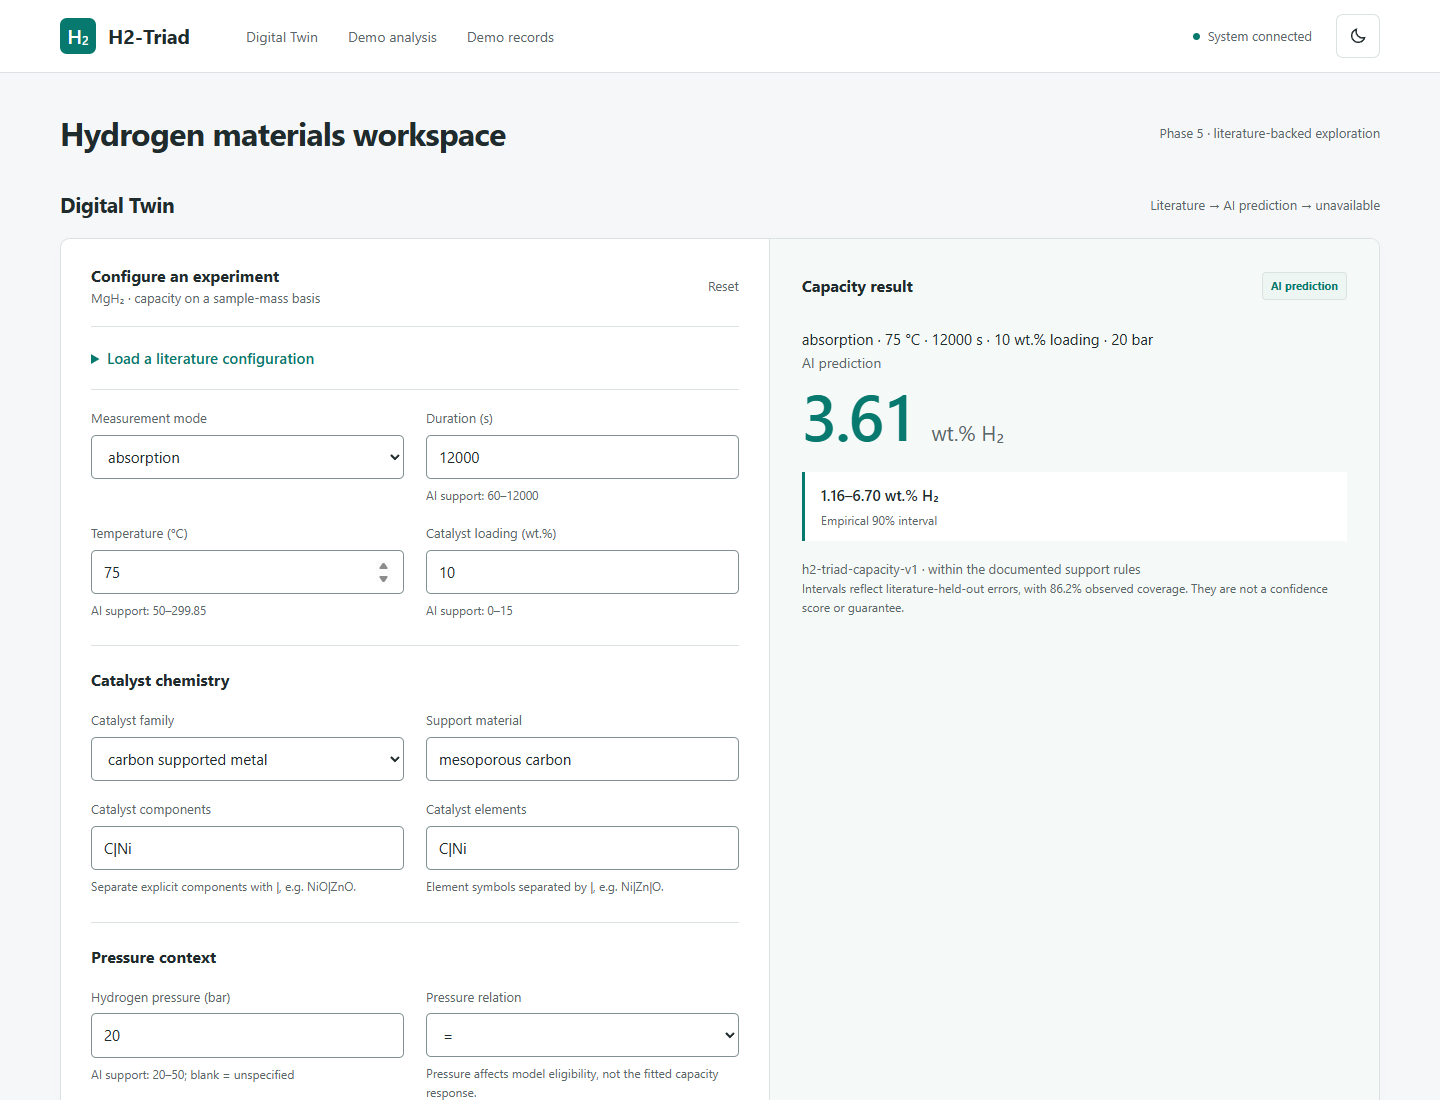
\includegraphics[width=\linewidth,height=0.43\textheight,keepaspectratio]{digital-twin.png}
  \caption{The H2-Triad Digital Twin configured for a supported absorption estimate. The interface keeps the submitted conditions, model result, empirical interval, and support status visible together.}
  \label{fig:digital-twin}
\end{figure}

\section{Response Landscape}

For a supported configuration, the application can evaluate a two-dimensional grid of temperature and catalyst loading while keeping all other inputs fixed. The resulting three-dimensional view uses temperature ($^{\circ}$C) and loading (\wtpct{}) as horizontal axes and predicted capacity (\wtpct{} \Htwo{}) as the vertical response. A separate prediction marks the exact selected configuration rather than estimating its value from a nearby grid node.

Every cell is validated before inference. Unsupported cells carry null capacity and interval values and remain excluded from the surface. The accessible grid table retains cell-level values, intervals, and masking reasons. This behavior preserves the boundary between learned response and unsupported space.

\begin{figure}[H]
  \centering
  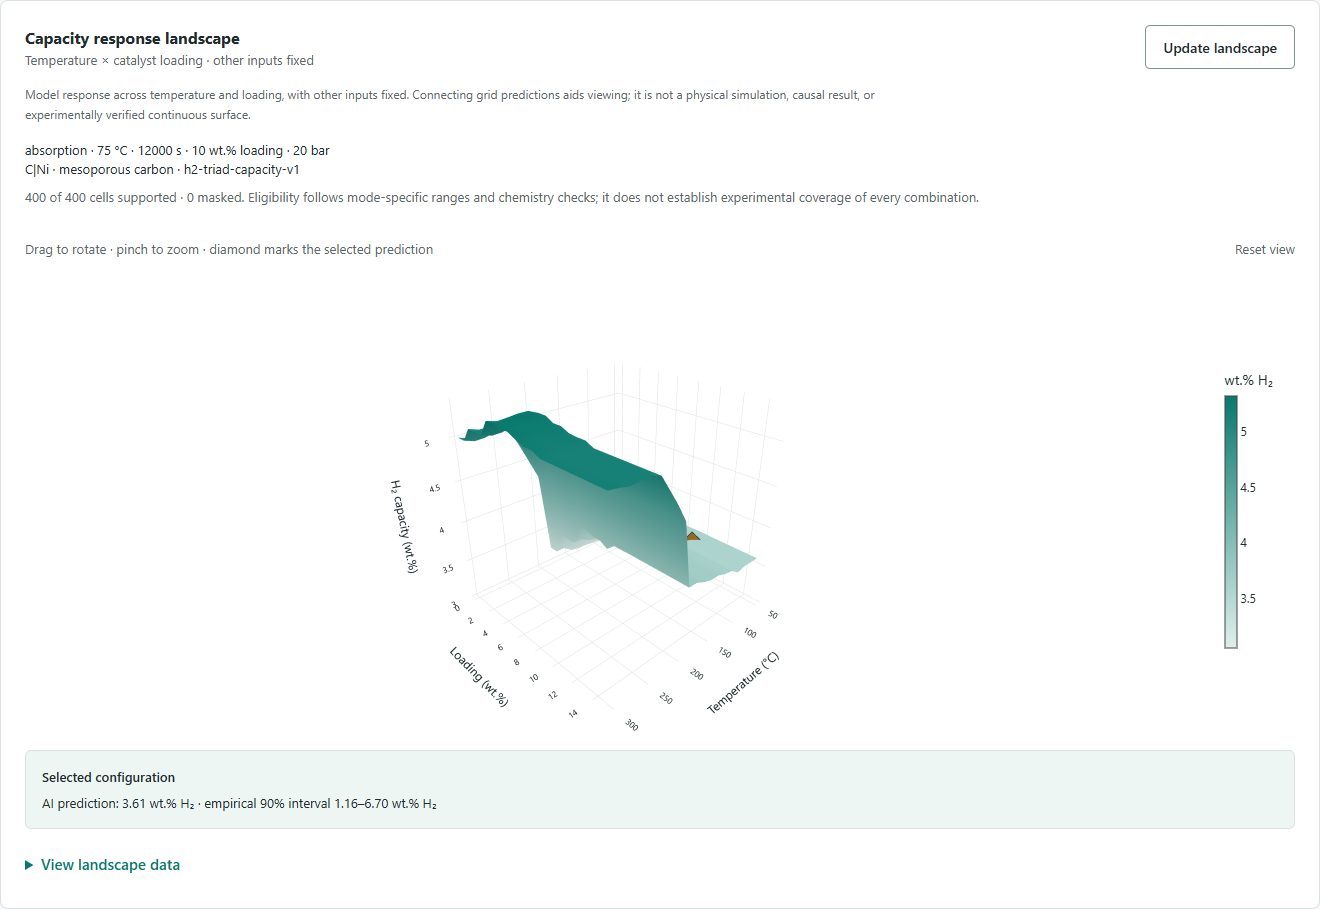
\includegraphics[width=\linewidth,height=0.40\textheight,keepaspectratio]{prediction-landscape.png}
  \caption{Implemented temperature $\times$ catalyst-loading response landscape with other conditions fixed. The surface visualizes the learned CatBoost response over supported grid cells; it is not a molecular model, physical simulation, causal result, or experimentally verified continuous surface.}
  \label{fig:landscape}
\end{figure}

\section{System Architecture and Deployment}

H2-Triad uses a React/Vite frontend and FastAPI backend. The backend connects the user-facing workflow to two deliberately distinct data paths: canonical literature tables and the cached CatBoost capacity predictor for scientific results, and a SQLite store for historical synthetic/demo exploration.

The production flow is compact:

\begin{center}
\small
\textbf{React/Vite interface} $\rightarrow$ \textbf{FastAPI service} $\rightarrow$
\begin{tabular}[t]{l}
canonical literature index \\
cached CatBoost predictor \\
SQLite synthetic/demo explorer
\end{tabular}
\end{center}

The repository-root Dockerfile is the production deployment path. A Node 24 build stage compiles the React application; a Python 3.10 slim runtime then serves both the bundled single-page application and the \texttt{/api} routes through one Uvicorn process. The container is deployed as one Railway service with same-origin API requests. The public deployment is available at \href{https://hydrax-h2-triad.up.railway.app}{hydrax-h2-triad.up.railway.app}.

\section{Current Validation}

Release validation covers model behavior, backend contracts, browser workflows, scientific data integrity, and integrated container operation. Recorded checks include 22 model tests, 72 backend tests, and 26 browser tests, with the browser suite also passing against the integrated container. Scientific checks preserve the 119-observation literature index, exact-measurement precedence, qualified values, unavailable responses without numeric fields, batched landscape masking, and stable production artifacts. The current implementation is a functioning, publicly deployed prototype rather than a proposal represented only through mockups.

\section{Limitations}

The following limitations govern interpretation:

\begin{itemize}
  \item The evidence base is small at the independent-paper level and is concentrated in particular journals and catalyst families.
  \item Paper-held-out performance is moderate, and the broad empirical intervals expose substantial uncertainty.
  \item Support rules are conservative feature-wise checks, not proof of dense joint experimental coverage.
  \item Generalization to unfamiliar chemistry is limited even when a warning-bearing prediction is permitted.
  \item No independent laboratory campaign, temporal validation, or external material system validates the model.
  \item Predictive associations and response plots do not establish causal optimization or physical mechanism.
\end{itemize}

The system is intended to support expert comparison, hypothesis prioritization, and transparent exploration. Scientific conclusions still require source review and laboratory confirmation.

\section{Expected Value for the Hackathon}

The project is submitted for organizer review as an implemented technical concept that can be demonstrated at the October Energy Hackathon. It offers judges and participants a concrete way to inspect how evidence-grounded AI can support materials exploration while preserving a visible boundary between reported results, model estimates, and unsupported configurations.

For a showcase or technical presentation, the live prototype supports a clear end-to-end demonstration: configure an \MgHtwo{} experiment, retrieve an exact literature result or obtain a bounded model estimate, inspect uncertainty and provenance, and explore a masked temperature--loading response landscape. The value is the integration of these functions into one transparent workflow, not a claim that the prototype has completed laboratory development or established an optimized catalyst.

\section{Conclusion}

HydraX Tri-Interface Catalyst, implemented through H2-Triad, creates a practical bridge between scattered \MgHtwo{} experimental literature and condition-aware predictive exploration. Its main contribution is not a claim of comprehensive materials simulation; it is an evidence-conscious workflow that keeps exact observations, supported estimates, uncertainty, provenance, and unsupported regions visibly distinct. Within the limits of the current dataset, the deployed prototype demonstrates how literature curation and bounded machine learning can support technical exploration without obscuring where experimental evidence ends. It is presented for hackathon approval and demonstration as a working project concept, not as a completed research publication.

\end{document}
